\chapter{Procedure}

\section{AC Sweep/Noise Analysis}

\begin{figure}[h]
    \centering
    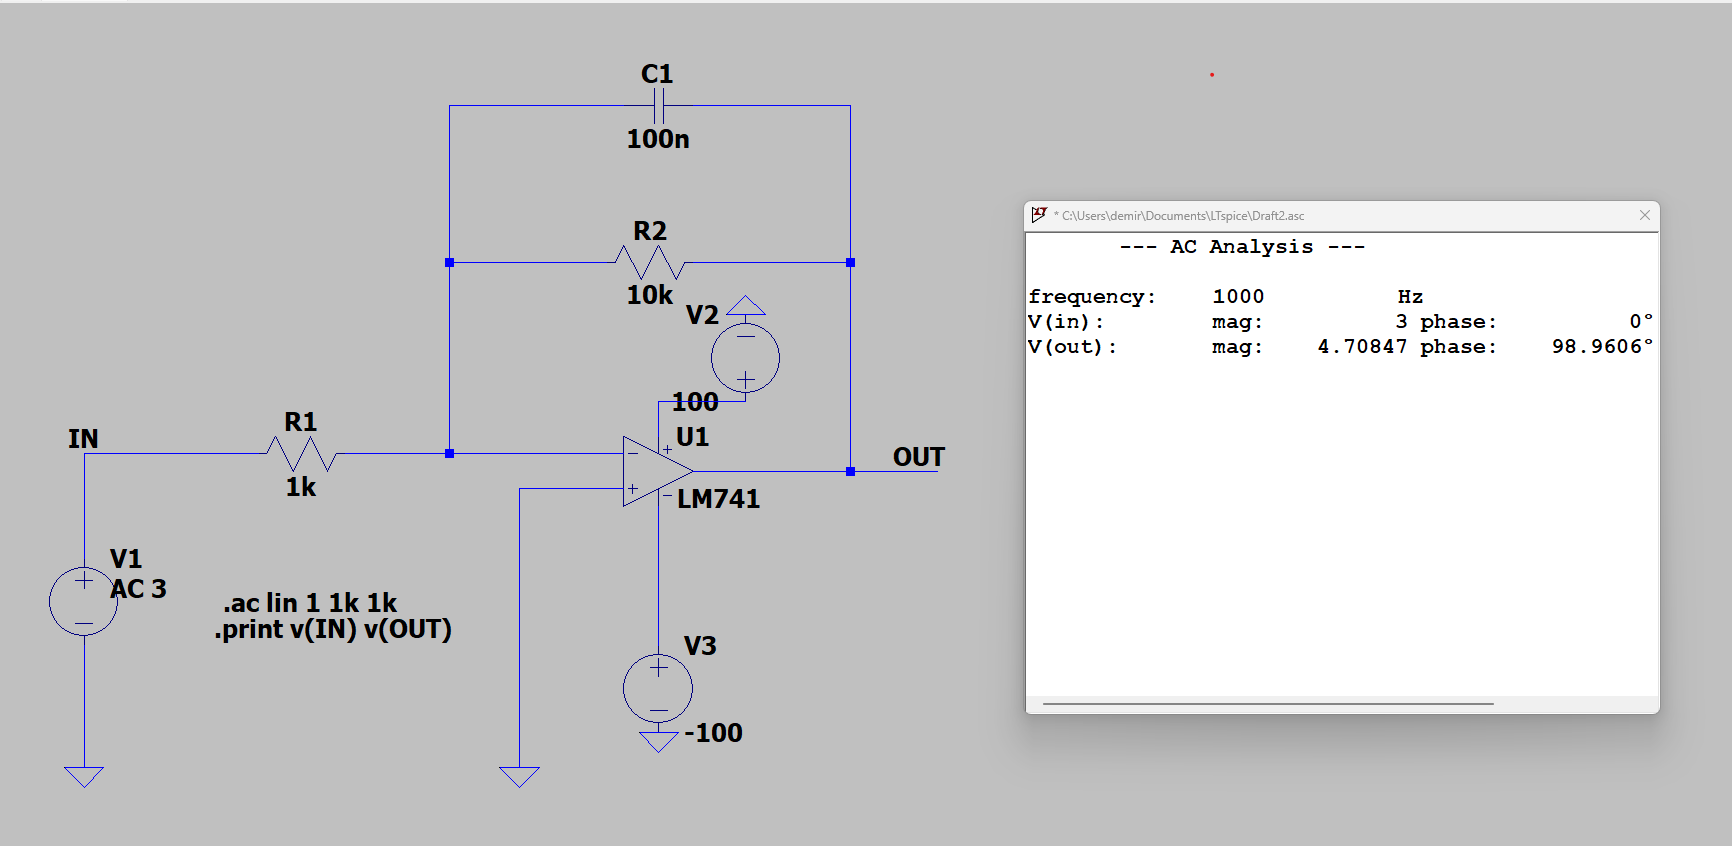
\includegraphics[width=0.6\textwidth]{assets/p1-1k.png}
    \caption{AC Analysis Circuit}
    \label{fig:ac-analysis-circuit}
|\end{figure}

\begin{table}[h]
    \centering
    \begin{tabular}{llll}
    \cline{1-2}
    \multicolumn{1}{|l|}{Frequency} & \multicolumn{1}{l|}{1kHz} &             &                              \\ \hline
    \multicolumn{1}{|l|}{$V_{in}$}     & mag: 3                    & phase: $0^{\circ}$    & \multicolumn{1}{l|}{} \\ \hline
    \multicolumn{1}{|l|}{$V_{out}$}    & mag: 4.70847               & phase: $98.96^{\circ}$ & \multicolumn{1}{l|}{} \\ \hline
                                    &                           &             &                             
    \end{tabular}
    \caption{AC Analysis Results}
    \label{tab:ac-sweep-analysis-results}
\end{table}

From the results, we can make these observations:

\begin{itemize}
    \item \textbf{Magnitude:} The gain og the circuit is approximately $1.57$ at $1kHz$. 
    \item \textbf{Phase:} The input signal has a phase of $0^{\circ}$, while the output signal exhibits a phase shift of $98.96^{\circ}$. This significant phase shift is typical in op-amp circuits operating at high frequencies. As the frequency increases, op-amps tend to introduce phase shifts due to internal capacitances and feedback delays. A shift of approximately 99° suggests that the circuit is approaching the higher end of the op-amp’s bandwidth, which leads to a lag in the output signal.
\end{itemize}

\newpage{}
\thispagestyle{plain}

\section{Frequency Response Analysis}

\begin{figure}[h]
    \centering
    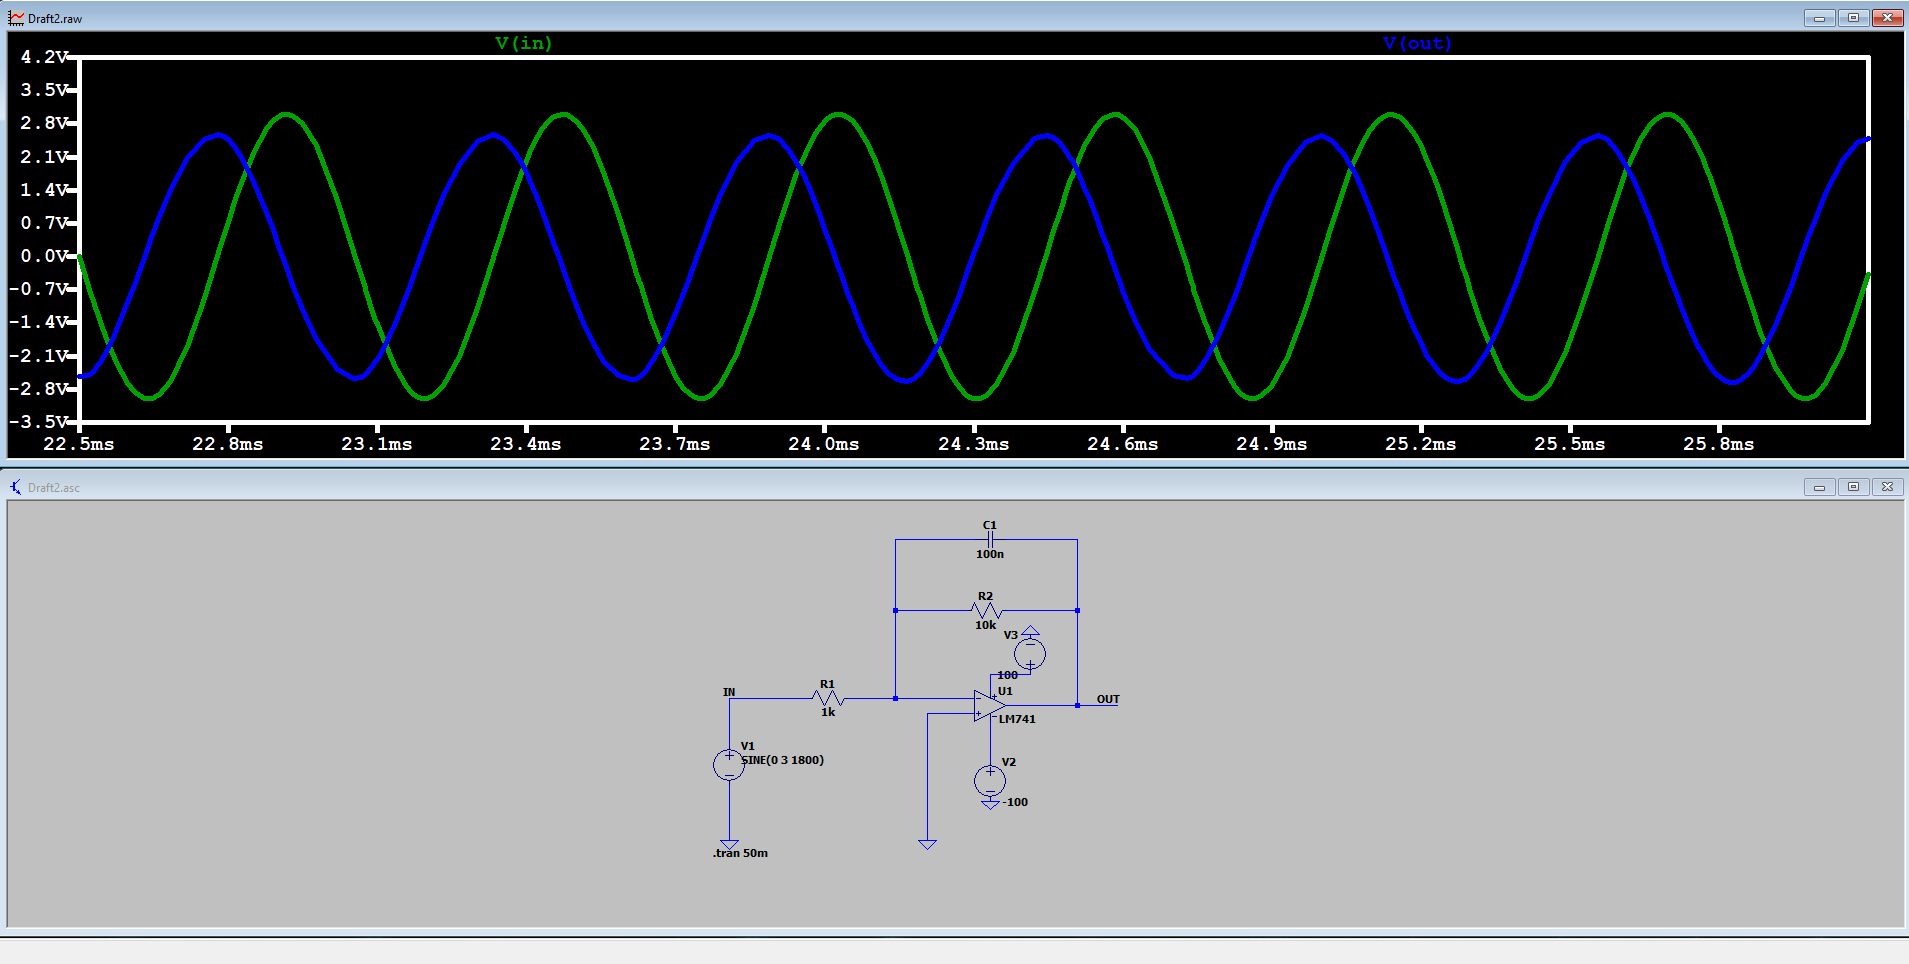
\includegraphics[width=0.8\textwidth]{assets/p2-1.8k.png}
    \caption{Frequency Response Analysis Circuit @ 1.8kHz}
    \label{fig:frequency-response-analysis-circuit-1.8k}
\end{figure}

\begin{figure}[h]
    \centering
    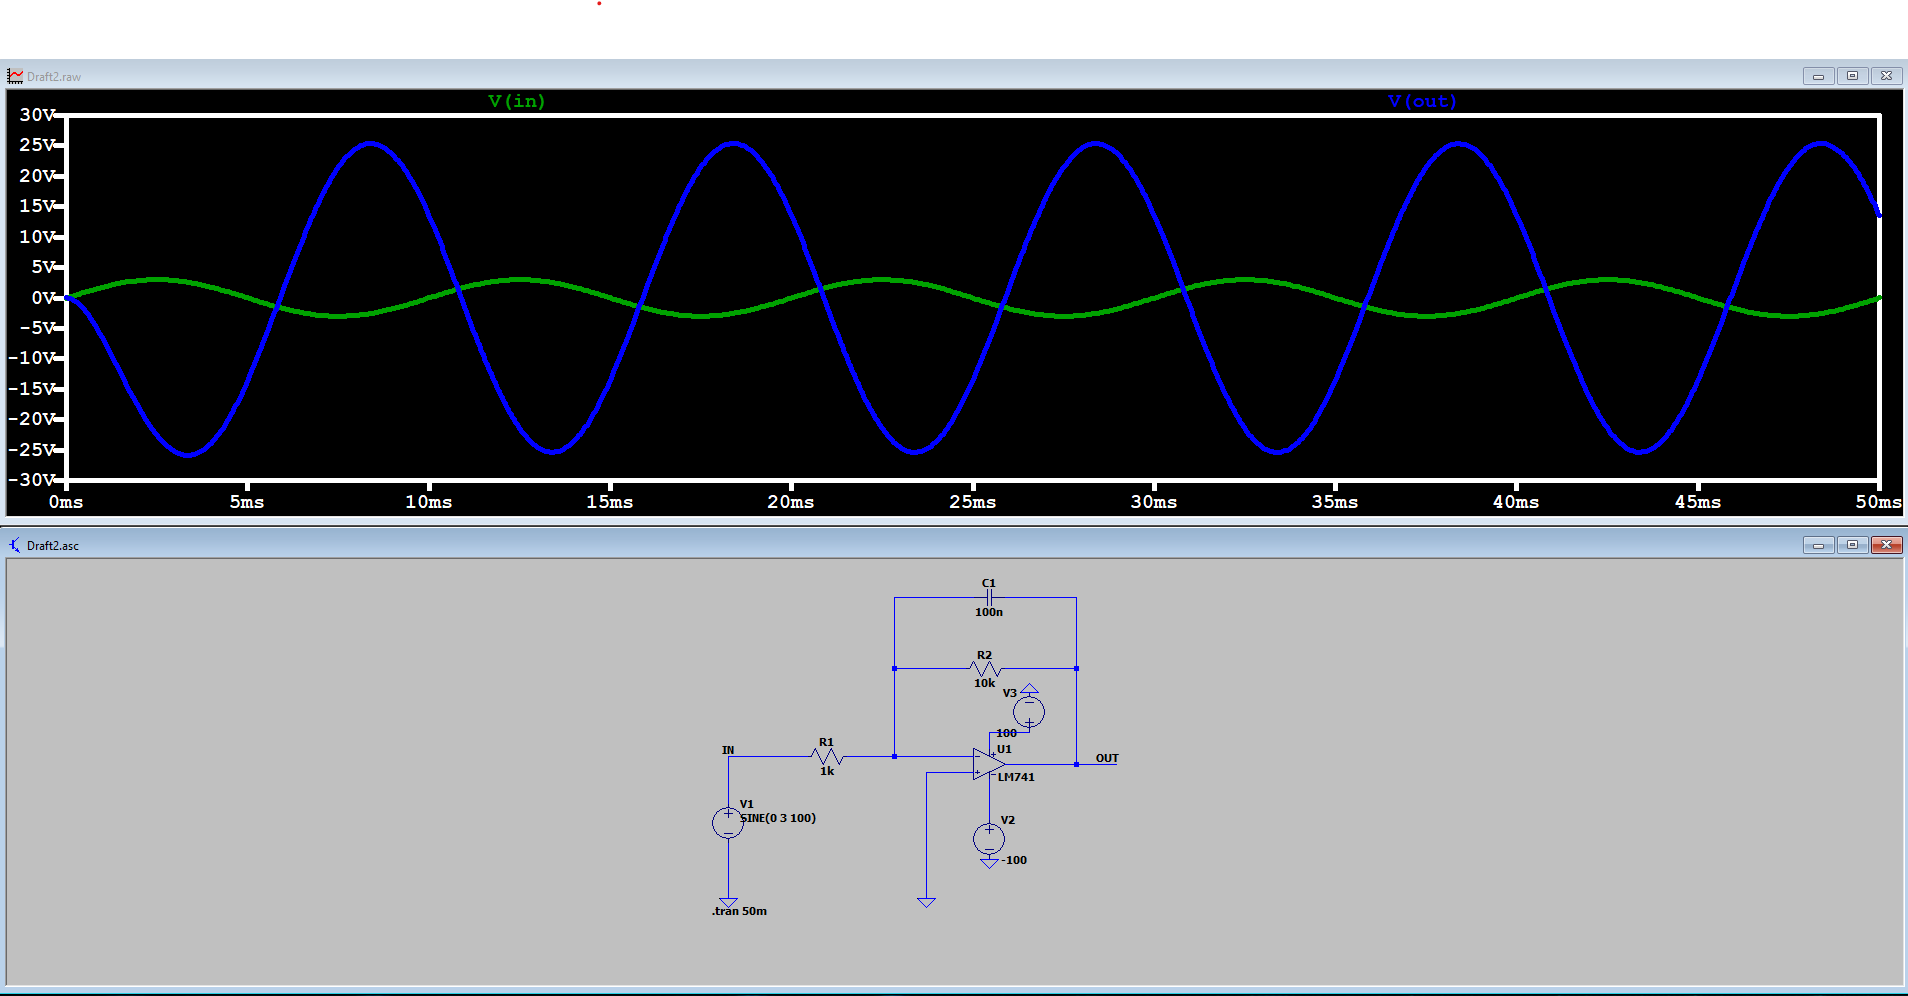
\includegraphics[width=0.8\textwidth]{assets/p2-100.png}
    \caption{Frequency Response Analysis Circuit @ 100Hz}
    \label{fig:frequency-response-analysis-circuit-100}
\end{figure}

At lower frequencies, op-amp behaves as expected. However, at higher frequencies, output starts to lag behing the input due to phase shifts, and the amplitude decreases, indicating a drop in gain as the op-amp bandwidth is exceeded.

\newpage{}
\thispagestyle{plain}

\section{Non-Inverting Amplifier Design}
For non-inverting amplifier design, we need to calculate the resistor values for the desired gain. The formula for calculating the resistor values is given below:

\begin{align*}
    4 = 1 + \frac{R_{f}}{R_{1}} &\Rightarrow \frac{R_{f}}{R_{1}} = 3 \\
    R_{f} &= 3k\Omega, R_{1} = 1k\Omega
\end{align*}

\begin{figure}[h]
    \centering
    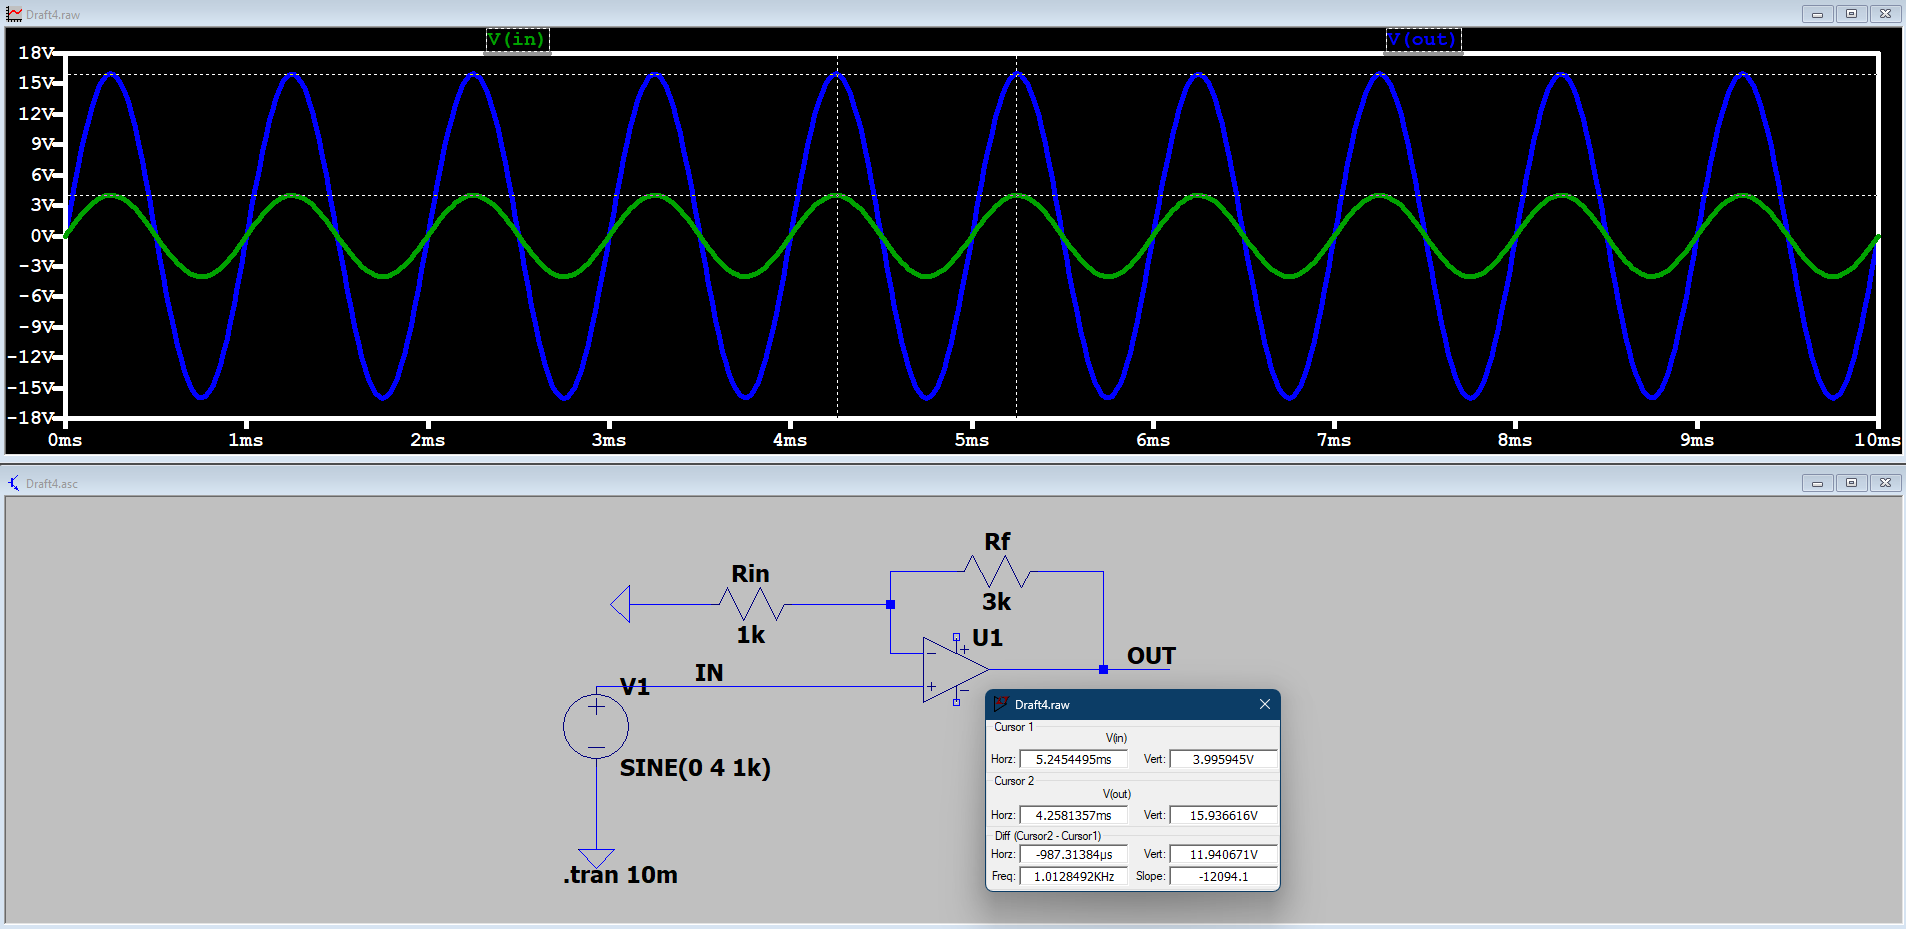
\includegraphics[width=0.8\textwidth]{assets/a4_design.png}
    \caption{Non-Inverting Amplifier Circuit @ 4V1kHz}
    \label{fig:non-inverting-amplifier-circuit-4v}
\end{figure}

\begin{figure}[h]
    \centering
    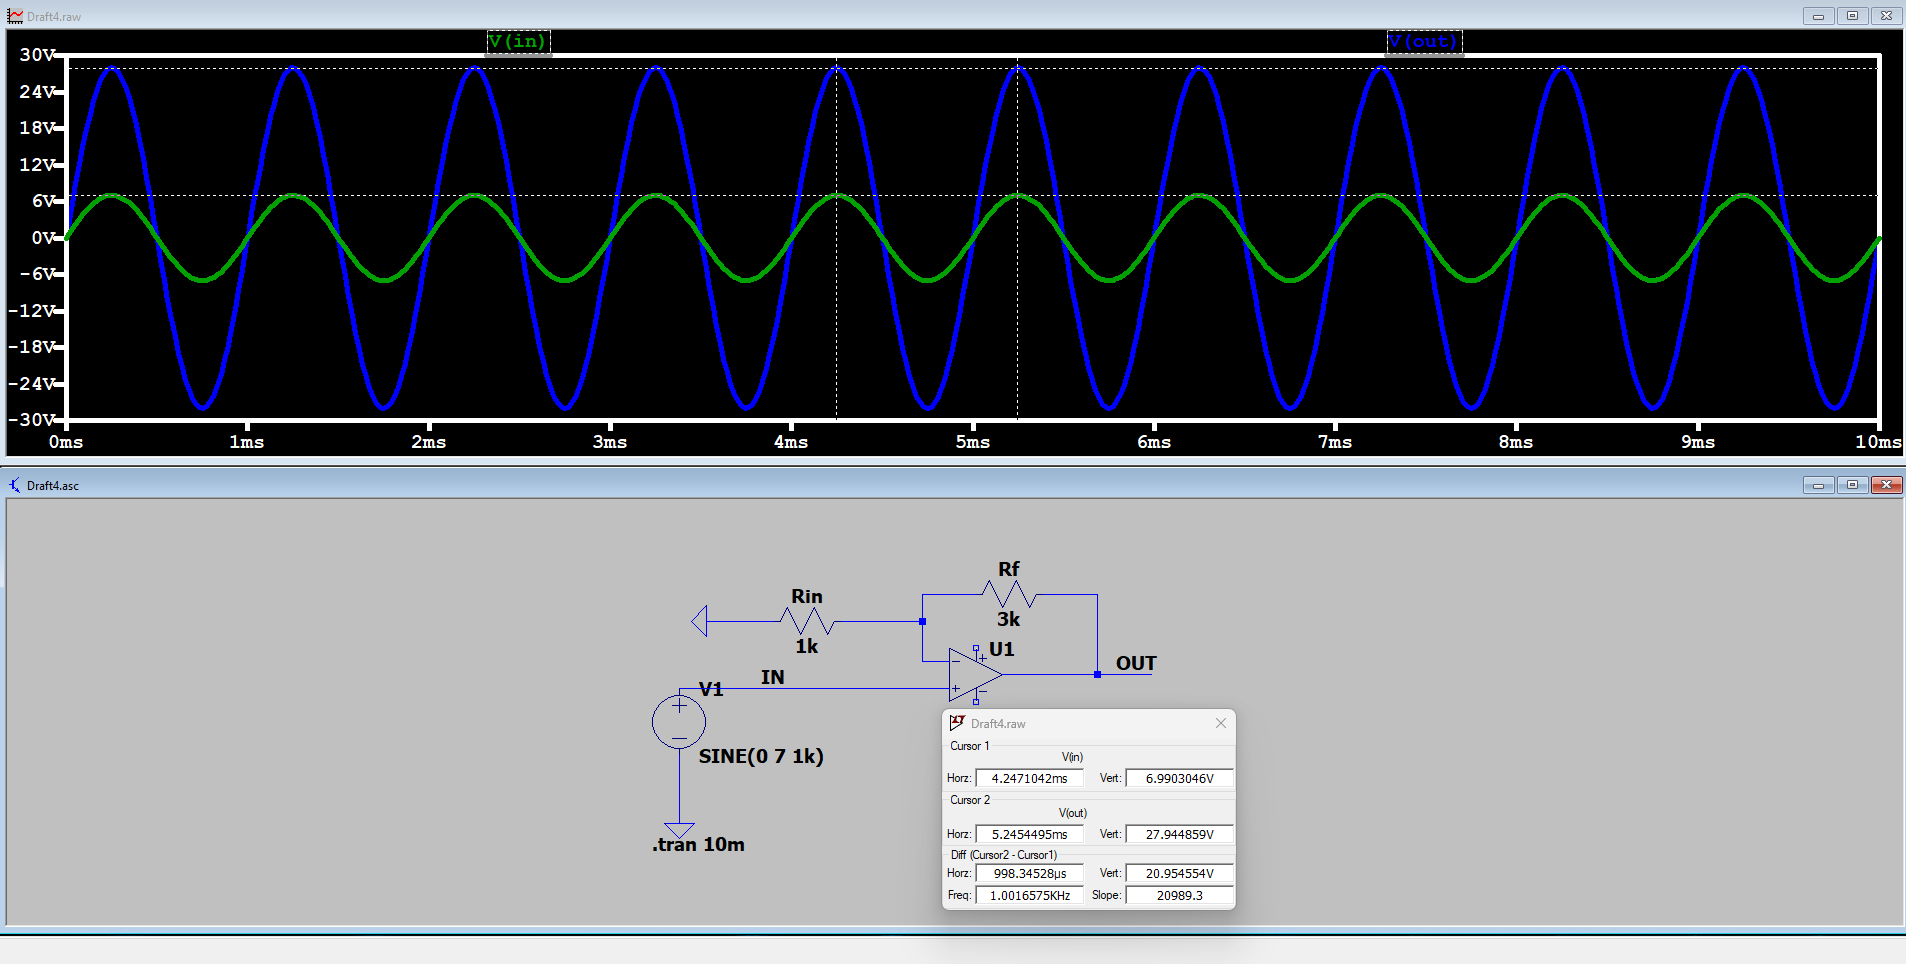
\includegraphics[width=0.8\textwidth]{assets/7_design.png}
    \caption{Non-Inverting Amplifier Circuit @ 7V1kHz}
    \label{fig:non-inverting-amplifier-circuit-7v}
\end{figure}

As we increase the voltage, the output voltage also increases. This is because the gain of the circuit is $4$.
